\documentclass[conference]{IEEEtran}
\IEEEoverridecommandlockouts

\usepackage{cite}
\usepackage{amsmath,amssymb,amsfonts}
\usepackage{algorithmic}
\usepackage{graphicx}
\usepackage{textcomp}
\usepackage{xcolor}
\usepackage{booktabs}
\usepackage{array}
\usepackage{tikz}
\usepackage{url}
% Character protrusion and font expansion. Materially improves justification in
% IEEEtran's narrow two-column measure, which is where nearly all the
% underfull-box warnings came from.
\usepackage{bbm}          % \mathbbm{1}: amssymb's \mathbb has no digits
\usepackage{microtype}
\usepackage[hidelinks]{hyperref}
\usetikzlibrary{positioning,arrows.meta,shapes.geometric,backgrounds,fit,calc}

\graphicspath{{../figures/}}
% Generated by run_all.py from named measurement records.
\newcommand{\RepeatThreeSpeed}{196.4}
\newcommand{\RepeatThreePower}{204.6}
\newcommand{\RepeatThreeTime}{1.61}
\newcommand{\RepeatThreeEnergy}{0.091}
\newcommand{\RepeatThreeMin}{0.078}
\newcommand{\RepeatThreeMax}{0.094}
\newcommand{\RepeatThreeMilliWh}{0.30}
\newcommand{\RepeatThreeHostZero}{0.091}
\newcommand{\RepeatThreeHostThirty}{0.12}
\newcommand{\RepeatThreeHostSixty}{0.13}
\newcommand{\RepeatThreeHostHundred}{0.15}
\newcommand{\RepeatEightSpeed}{102.5}
\newcommand{\RepeatEightPower}{222.2}
\newcommand{\RepeatEightTime}{3.09}
\newcommand{\RepeatEightEnergy}{0.19}
\newcommand{\RepeatEightMin}{0.17}
\newcommand{\RepeatEightMax}{0.20}
\newcommand{\RepeatEightMilliWh}{0.63}
\newcommand{\RepeatEightHostZero}{0.19}
\newcommand{\RepeatEightHostThirty}{0.24}
\newcommand{\RepeatEightHostSixty}{0.27}
\newcommand{\RepeatEightHostHundred}{0.31}
\newcommand{\RtxThreeSpeed}{195.6}
\newcommand{\RtxThreePower}{203.4}
\newcommand{\RtxThreeTime}{1.62}
\newcommand{\RtxThreeEnergy}{0.091}
\newcommand{\RtxThreeMin}{0.078}
\newcommand{\RtxThreeMax}{0.093}
\newcommand{\RtxThreeMilliWh}{0.30}
\newcommand{\RtxThreeHostZero}{0.091}
\newcommand{\RtxThreeHostThirty}{0.12}
\newcommand{\RtxThreeHostSixty}{0.13}
\newcommand{\RtxThreeHostHundred}{0.15}
\newcommand{\RtxEightSpeed}{101.8}
\newcommand{\RtxEightPower}{224.1}
\newcommand{\RtxEightTime}{3.11}
\newcommand{\RtxEightEnergy}{0.19}
\newcommand{\RtxEightMin}{0.18}
\newcommand{\RtxEightMax}{0.19}
\newcommand{\RtxEightMilliWh}{0.65}
\newcommand{\RtxEightHostZero}{0.19}
\newcommand{\RtxEightHostThirty}{0.24}
\newcommand{\RtxEightHostSixty}{0.27}
\newcommand{\RtxEightHostHundred}{0.31}
\newcommand{\AdaptationBaseAccuracy}{86.7}
\newcommand{\AdaptationAdaptedAccuracy}{97.8}
\newcommand{\AdaptationFrontierAccuracy}{95.0}
\newcommand{\AdaptationUplift}{11.1}
\newcommand{\AdaptationUpliftLow}{5.0}
\newcommand{\AdaptationUpliftHigh}{18.3}
\newcommand{\AdaptationClusterP}{0.250}
\newcommand{\AdaptationObservationCount}{300}
\newcommand{\AdaptationModelCount}{3}
\newcommand{\AdaptationExtractionBaseAccuracy}{100.0}
\newcommand{\AdaptationExtractionAdaptedAccuracy}{100.0}
\newcommand{\AdaptationExtractionUplift}{0.0}
\newcommand{\AdaptationExtractionP}{1.000}
\newcommand{\AdaptationExtractionAdjustedP}{1.000}
\newcommand{\AdaptationRagBaseAccuracy}{100.0}
\newcommand{\AdaptationRagAdaptedAccuracy}{100.0}
\newcommand{\AdaptationRagUplift}{0.0}
\newcommand{\AdaptationRagP}{1.000}
\newcommand{\AdaptationRagAdjustedP}{1.000}
\newcommand{\AdaptationSummaryBaseAccuracy}{91.7}
\newcommand{\AdaptationSummaryAdaptedAccuracy}{100.0}
\newcommand{\AdaptationSummaryUplift}{8.3}
\newcommand{\AdaptationSummaryP}{1.000}
\newcommand{\AdaptationSummaryAdjustedP}{1.000}
\newcommand{\AdaptationSimpleCodeBaseAccuracy}{91.7}
\newcommand{\AdaptationSimpleCodeAdaptedAccuracy}{100.0}
\newcommand{\AdaptationSimpleCodeUplift}{8.3}
\newcommand{\AdaptationSimpleCodeP}{1.000}
\newcommand{\AdaptationSimpleCodeAdjustedP}{1.000}
\newcommand{\AdaptationHardReasonBaseAccuracy}{50.0}
\newcommand{\AdaptationHardReasonAdaptedAccuracy}{88.9}
\newcommand{\AdaptationHardReasonUplift}{38.9}
\newcommand{\AdaptationHardReasonP}{0.250}
\newcommand{\AdaptationHardReasonAdjustedP}{1.000}
\newcommand{\AdaptationHoldoutBaseAccuracy}{80.0}
\newcommand{\AdaptationHoldoutAdaptedAccuracy}{90.0}
\newcommand{\AdaptationHoldoutFrontierAccuracy}{95.0}
\newcommand{\AdaptationHoldoutUplift}{10.0}
\newcommand{\AdaptationHoldoutUpliftLow}{5.0}
\newcommand{\AdaptationHoldoutUpliftHigh}{15.0}
\newcommand{\AdaptationHoldoutClusterP}{0.250}
\newcommand{\AdaptationSemanticBaseAccuracy}{90.3}
\newcommand{\AdaptationSemanticAdaptedAccuracy}{91.8}
\newcommand{\AdaptationSemanticFrontierAccuracy}{95.0}
\newcommand{\AdaptationSemanticUplift}{1.4}
\newcommand{\AdaptationSemanticUpliftLow}{-3.3}
\newcommand{\AdaptationSemanticUpliftHigh}{7.7}
\newcommand{\AdaptationSemanticClusterP}{1.000}


% PaperBanana-style palette
\definecolor{edgegreen}{HTML}{16A085}
\definecolor{edgedark}{HTML}{0E6E5C}
\definecolor{cloudorange}{HTML}{E8743B}
\definecolor{heavyred}{HTML}{C0392B}
\definecolor{accentblue}{HTML}{2F6FED}
\definecolor{ink}{HTML}{1F2933}
\definecolor{softbg}{HTML}{F4F7F6}
\definecolor{relaypurple}{HTML}{7A5BD8}

\newcommand{\Wh}{\,\text{Wh}}
\newcommand{\mL}{\,\text{mL}}
\newcommand{\gco}{\,\text{gCO\textsubscript{2}e}}
\newcommand{\fs}{f_{s}}

\begin{document}

\title{Right-Sized AI at the Edge:\\
Quantifying Carbon, Water, Cost, and Capability in\\
Peer-to-Peer Inference}

\author{\IEEEauthorblockN{AutoYou Research}
\IEEEauthorblockA{\textit{Decentralized Inference \& Sustainable Compute Group}\\
\texttt{research@autoyou.me}}}

\maketitle

\begin{abstract}
Data-centre electricity demand is projected to more than double to
approximately 945\,TWh by 2030, about the consumption of Japan, driven chiefly
by AI inference. A widely proposed remedy is to decentralize it: run small
language models (SLMs) on already-owned consumer hardware, connect peers
directly over WebRTC, and call frontier cloud models only when a task truly
needs them. We ask when this helps and when it does not. We build a
parameter-driven model of per-query energy, water, carbon and cost, grounded in
public measurements, published estimates and explicit sensitivity ranges, with a
fleet-scale extrapolation on the IEA 2030 base and a 50{,}000-draw Monte-Carlo
with one-at-a-time sensitivity analysis; six hypotheses and three counter-claims
each receive a validated, partial or refuted verdict.

The central result is scoped. For the capability-sufficient fraction of a
representative assistant workload - approximately 82\% at a 70\% acceptance
threshold, which sits \emph{above} NVIDIA's measured 40--70\% agentic-replaceability
range because our workload mix is an authorial assumption rather than a sampled
corpus - edge execution cuts per-query carbon by $54$--$64\%$ against typical and
heavy frontier usage with positive savings in all Monte-Carlo draws, nearly
eliminates on-site cooling water, and costs approximately 150 times less per
query. The unqualified claim fails against a best-in-class efficient cloud
model: compared with Gemini's 0.24\,Wh/prompt a single-user consumer GPU is on
average 16\% worse, with positive savings in only 3\% of draws. The win
therefore comes from right-sizing, from eliminating evaporative cooling and
PUE/idle overhead ($42\%$ of a hyperscaler's measured per-prompt footprint), and
from using marginal energy on existing hardware - not from relocating the same
model. The benefit is grid-conditional, survives induced usage growth up to
approximately 212\% -- equivalently, take-back of the entire gross saving, the
two being one model in two units -- and WebRTC DTLS preserves transport
confidentiality against
STUN/TURN relays by construction.

Two further passes test this model where it is weakest. A companion study
\cite{autoyou2026adaptation} relaxes its central simplification, that per-class
capability is fixed by parameter count, and finds $\fs$ unchanged at an ordinary
acceptance threshold. A primary measurement campaign across two consumer hardware
platforms - an AMD Radeon 8060S APU (64\,GB unified memory) and an NVIDIA GeForce
RTX 5070 discrete GPU (12\,GB GDDR7) - grounds the edge decode, prefill, and
energy terms in direct observation. On the APU, single-stream generation reaches
78.4, 37.8, and 13.8\,tok/s for 3.8B, 8.9B, and 27.3B models, with prompt
regressions revealing prefill ratios of $0.050$--$0.078$. A nine-build bandwidth
ladder supports the memory-bound decode premise only in its ordering: builds that
stream every weight sit below builds that provably do not, by $30$ percentage
points, but the whole-weight class spans $77$--$106\%$ of the specified ceiling
rather than a tight band. One dense build exceeds a ceiling no whole-file reader
can exceed, which measures the error in the $\tau\!\cdot\!W$ proxy rather than
the hardware and bounds how tightly the statistic can be read. On the discrete
GPU, sampled board telemetry measures request-window energy at \RtxThreeEnergy{}\Wh\
(3B) and \RtxEightEnergy{}\Wh\ (8B) at 499 prompt and 300 output tokens, replicated
at \RepeatThreeEnergy{}\Wh\ and \RepeatEightEnergy{}\Wh; two significant figures
is all the instrument supports. Host-power sensitivities are evaluated up to
100\,W. The models, datasets, telemetry harnesses, and an empirical routing agent
are released openly, and every measured row is reported rather than
filtered.
\end{abstract}

\begin{IEEEkeywords}
sustainable AI, edge inference, small language models, agentic AI, WebRTC,
peer-to-peer, data-centre water, carbon footprint, total cost of ownership,
Jevons paradox.
\end{IEEEkeywords}

\section{Introduction}
The marginal cost of an AI answer is no longer purely computational; it is
environmental and economic. The IEA projects global data-centre electricity
demand to \textbf{more than double to \textasciitilde945\,TWh by 2030}, with
AI-optimised facilities quadrupling and the United States alone accounting for
nearly half of the growth \cite{iea2025}. Per query, a median Gemini text prompt
is measured at $0.24\Wh$, $0.26\mL$ water, $0.03\gco$ \cite{elsworth2025}; an
independent benchmark places a short GPT-4o query at $0.42\Wh$ and a single long
reasoning query (o3, DeepSeek-R1) above $30\Wh$ \cite{jegham2025}. Yet
data-centre power-usage effectiveness (PUE) has been stuck at a global average of
$1.54$ for six years \cite{uptime2025}. Reported water-use effectiveness spans
from best-in-class hyperscale operation near $0.12$\,L/kWh to an industry
withdrawal-WUE benchmark around $0.84$\,L/kWh, with high-water facilities above
$1$\,L/kWh \cite{aws_water2025,devriesgao2025}.

A decentralized alternative is increasingly credible. NVIDIA Research recently
argued that \emph{small language models are the future of agentic AI}: SLMs are
``sufficiently powerful, inherently more suitable, and necessarily more
economical'' for most agentic invocations, and \emph{heterogeneous} systems that
mix SLMs with occasional frontier calls are the natural design \cite{belcak2025}.
They report SLMs matching far larger models: Phi-2 (2.7B) reaching 30B-class
commonsense and code at $\sim$15$\times$ the speed, SmolLM2 (1.7B) matching 14B
peers on tool-calling and instruction-following, and xLAM-2-8B \emph{surpassing}
GPT-4o and Claude-3.5 on tool calling. They also measure that $40$--$70\%$ of
LLM calls in real agentic systems (MetaGPT, Open Operator, Cradle) are
SLM-replaceable.

This paper adds a \emph{quantitative environmental,
economic, and capability model} for decentralizing such inference to peers'
own devices over relay-confidential transport, with explicit boundary
conditions. The \emph{reference architecture} we model throughout is assembled
entirely from public components: WebRTC SCTP-over-DTLS transport, STUN-first NAT
traversal with geo-spread TURN fallback, and a local-first SLM runtime
(Ollama/LiteLLM serving Ministral- and Llama-class 3B--8B builds) with an
operator-selectable multi-provider cloud path (OpenAI, Anthropic, Google). We
describe it not as a system contribution but as the concrete configuration the
model's parameters refer to, so that every term in the analysis has an
unambiguous physical referent. Every quantitative input is drawn from a public
cited source or an explicit modelling assumption varied in sensitivity analysis;
no proprietary component is required to reproduce any result reported here.

\textbf{Contributions.}
(1) A parameter-driven model of per-query \emph{energy, water,
carbon, and cost} for cloud-frontier vs.\ edge-SLM inference, plus P2P transport
(\S\ref{sec:methodology}).
(2) A capability-sufficiency formulation tied to current public benchmarks and
read against NVIDIA's measured agentic-replaceability rates, which it exceeds
(\S\ref{sec:results}).
(3) A \emph{fleet-scale} extrapolation on the IEA 2030 inference base, and a
\emph{total-cost-of-ownership} comparison (\S\ref{sec:results}).
(4) Six falsifiable hypotheses and three counter-claims, each with an explicit
verdict backed by a 50k-draw Monte-Carlo and a sensitivity tornado, including an
explicit account of \emph{where the thesis fails} (\S\ref{sec:threats}).
(5) A reproducible open harness and a runnable agent that executes the derived
routing rule live.
(6) \emph{Primary measurement} of single-stream inference on two consumer
platforms, a unified-memory APU and a discrete GPU (\S\ref{sec:measured}),
which replaces two of the three borrowed terms in the edge-energy model with
measured ones and puts the bandwidth-bound premise behind the device-class
argument to a test it could fail --- and partly did.

We avoid claims outside the evidence. The contribution is the boundary conditions
under which decentralization helps, and the cases where it does not.

\section{Background and Related Work}
\textbf{The footprint of inference.}
PUE captures facility overhead (global $1.54$ \cite{uptime2025}; hyperscale
$1.09$--$1.15$). The EU Energy Efficiency Directive now mandates data-centre
reporting and is preparing a rating scheme and possible minimum performance
standards; we therefore do not model an EU-wide PUE cap \cite{eu_eed2026}. WUE
for on-site cooling varies widely: AWS reports $0.15$\,L/kWh for 2024, improving
to $0.12$ in 2025, and cites
an industry withdrawal-WUE benchmark of $0.84$\,L/kWh
\cite{aws_water2025,devriesgao2025}; off-site water embedded in generation is
separate and often larger \cite{ucriverside2023}; we carry it as an explicit
scenario parameter (EWIF, Table~\ref{tab:params}) with a wide range rather than a
cited point value, because published factors vary by generation mix and no
single figure fits a global average. Grid carbon intensity averages
$458\gco$/kWh
globally, spanning EU $\sim$140 to India $\sim$708 \cite{ember2026}. Jegham
\emph{et al.}\ \cite{jegham2025} benchmark per-query energy across model sizes;
Google \cite{elsworth2025} provide a comprehensive at-scale measurement showing
$42\%$ of the per-prompt footprint is \emph{non-compute} (CPU/DRAM $24\%$,
idle/redundancy/overhead $18\%$), a margin a household device does not pay.

\textbf{Small models, agentic systems.}
Surveys of SLMs \cite{wang2024slm} and the Ministral 3B/8B release
\cite{mistral2024} document 3B--8B models approaching frontier quality on
knowledge, coding, and grounded tasks while trailing on hard reasoning. NVIDIA's
agentic-SLM position paper \cite{belcak2025} crystallises this into a design
thesis: right-size each invocation and fall back to a frontier model only when
needed. It also supplies the capability and economic evidence we build on. Our work
is complementary: where \cite{belcak2025} argues capability and cost, we add the
\emph{environmental} model, the \emph{transport} layer, and a falsifiable
boundary analysis.

\textbf{The mid-2026 frontier.}
The frontier changed substantially between the measurement corpus above and the
present analysis. OpenAI released the GPT-5.6 family (Sol, Terra, and Luna) in
July 2026; Anthropic released Claude Sonnet 5 in June 2026 alongside the Fable 5
frontier tier; Google released Gemini 3.6 Flash in July 2026; and two
open-weights sparse mixture-of-experts flagships appeared, Moonshot AI's Kimi K3
(2.8T total parameters, 16 of 896 experts active per token) and Zhipu AI's
GLM-5.2 (744B total, approximately 40B active) \cite{frontier2026,anthropic_pricing2026,google_pricing2026,openweights2026}. Two
observations follow. First, no public per-query energy measurement covers these
models at the time of writing; the most recent measurement studies
\cite{jegham2025,caravaca2025} characterise earlier deployments. Our energy,
water, and carbon results are therefore pinned to measured models, and the 2026
roster enters the analysis through pricing and architecture alone
(\S\ref{sec:results}). Second, sparse expert activation is right-sizing
applied \emph{inside} the cloud model: per-token compute is decoupled from total
capacity. That reinforces the central H2 lever (\emph{which size runs}) and
enlarges, rather than shrinks, the efficient-cloud counter-case of H5.

\textbf{Edge inference and P2P transport.}
Edge execution can cut energy $65$--$90\%$ for suitable tasks
\cite{techtarget2025} --- a trade-press figure we carry for its direction
rather than its magnitude --- but consumer accelerators are less efficient
\emph{per token} than batched data-centre GPUs, because batching amortises one
pass over the weights across concurrent requests and single-stream execution
cannot. We make that tension explicit and quantify its mechanism, not its
ratio, in C2. WebRTC P2P succeeds directly for $\sim$70--85\% of
sessions via STUN, needing TURN relay for $\sim$10--20\% \cite{antmedia2026}; the
transport is DTLS-secured by mandate with SDP fingerprint pinning
\cite{rfc8831,rfc8827}, so relays forward only ciphertext. This is a
transport-layer statement: an authenticated peer is still an application-level
endpoint, not a privacy-preserving black box.

\textbf{Where the measurements are, and are not.}
Three bodies of work measure inference energy directly, and the gap between them
is what this paper's Pass 4 addresses. Jegham \emph{et al.} \cite{jegham2025}
benchmark per-query energy, water and carbon across model sizes on H100/H200
\emph{server} accelerators at batch 8. Elsworth \emph{et al.} \cite{elsworth2025}
report a comprehensive at-scale measurement of a production TPU fleet, and are
the only source we know of that closes the loop from accelerator to facility.
Caravaca \emph{et al.} \cite{caravaca2025} contribute over 32{,}500 GPU
inference-energy measurements and a predictive per-query model, again on
data-centre parts. All three measure the \emph{cloud} side.

The standardised counterpart is MLPerf Inference \cite{reddi2020mlperf}, which
defines the single-stream scenario we use and an edge division alongside its
datacentre one. Its submissions are vendor-run on curated systems and its edge
division has centred on embedded and automotive silicon; we are not aware of
results for a consumer unified-memory APU serving quantised LLMs through a
commodity runtime, which is the configuration a household actually has.

We are not aware of a comparable measurement of the \emph{consumer} side, and
that asymmetry has a consequence for every study of this kind: the cloud
baseline is measured while the edge baseline is extrapolated from vendor
specifications and enthusiast benchmarks. Ours was, until \S\ref{sec:measured}.
We report empirical measurements across two distinct consumer device classes: a
unified-memory APU (AMD Radeon 8060S with 64\,GB unified LPDDR5X) and a
high-bandwidth discrete GPU (NVIDIA GeForce RTX 5070 with 12\,GB GDDR7). These
provide execution throughput under commodity runtimes, a multi-architecture
bandwidth roofline evaluation, and direct sampled board-power integration.
The premise those numbers are used to test is not new in itself. That
memory-bound kernels are limited by operational intensity against a bandwidth
ceiling is the roofline model \cite{williams2009roofline}, and that
single-stream autoregressive decode sits on the memory-bound side of that roof
is widely assumed in systems work on LLM serving. What is usually missing is a
measurement of \emph{where under the roof} a consumer part actually lands when
running a commodity stack, across model families it was not tuned for. Reporting
that - and reporting the architectures that must and do sit above the roof - is
the contribution here. The scope is modest: one serving stack, two machines.

\textbf{The rebound risk.}
Efficiency can induce demand (Jevons' paradox); LLM rebound is estimated at
$15$--$25\%$ \cite{luccioni2025}, and embodied hardware carbon is $15$--$30\%$ of
data-centre emissions \cite{schneider2025}. We charge both against our savings.

\section{System Model and Reference Architecture}
\label{sec:architecture}
Figure~\ref{fig:arch} shows the decentralized data path. A query is classified;
a capability router sends it to a local SLM when the task is SLM-sufficient, an
edge device is available, and the local grid is below the routing crossover;
otherwise it routes to a cloud frontier provider. STUN establishes direct P2P for
the majority of sessions; a geographically co-located (e.g.\ ISP-edge) TURN relay
forwards \emph{ciphertext only} for the NAT-restricted minority. This is the
heterogeneous design advocated in \cite{belcak2025}, with the transport and
siting made concrete.

\textbf{Realization.} The architecture is realized across two
implemented components, and the analysis distinguishes them throughout. Transport and
local-first execution are provided by the platform server: datachannels run
SCTP-over-DTLS, NAT class is determined by STUN probing, and
operator-configured ICE servers are merged with short-lived TURN credentials
issued by a geographically aware credential service, degrading to local-only
configuration whenever that service is unreachable. Its default inference
provider is the on-device SLM runtime; cloud providers are configured
alternatives, reached either through a direct Gemini adapter or through a
LiteLLM adapter for OpenAI- and Anthropic-class models. Per-query capability
routing is provided by the reference agent. The division is
deliberate: the server treats a locally configured provider as binding and
performs no automatic escalation, so that no query leaves the device without an
explicit operator decision. The analytical consequence is direct. Results that
depend on routing the hard $(1-\fs)$ fraction to a frontier model characterize
the heterogeneous system as specified and as implemented in the agent, whereas
a default server deployment realizes the $\fs$ edge fraction and delegates
escalation to operator policy.

\begin{figure}[t]
\centering
\resizebox{\columnwidth}{!}{%
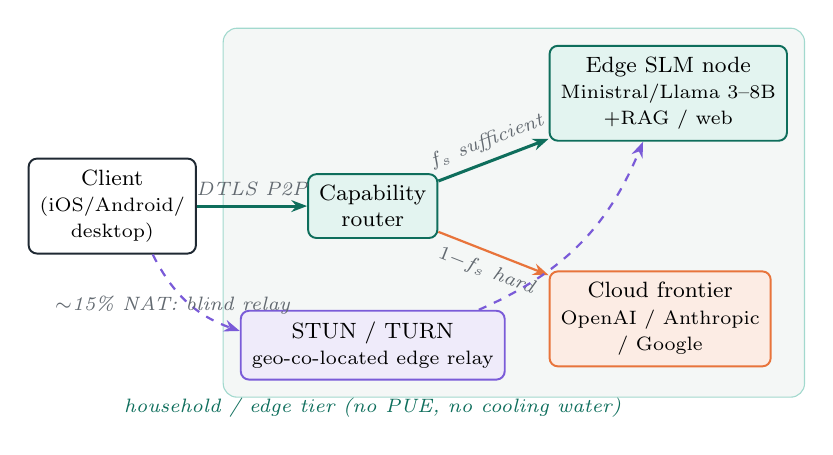
\begin{tikzpicture}[
  font=\footnotesize,
  box/.style={rounded corners=3pt, draw=ink, line width=0.7pt, align=center,
              inner sep=4pt, minimum height=8mm, fill=white},
  edgebox/.style={box, fill=edgegreen!12, draw=edgedark},
  cloudbox/.style={box, fill=cloudorange!14, draw=cloudorange},
  relaybox/.style={box, fill=relaypurple!12, draw=relaypurple},
  lbl/.style={font=\scriptsize\itshape, text=ink!70},
  flow/.style={-{Stealth[length=2mm]}, line width=0.8pt},
  dtls/.style={flow, edgedark, line width=1.1pt},
]
\node[box] (client) {Client\\ \scriptsize(iOS/Android/\\ \scriptsize desktop)};
\node[edgebox, right=14mm of client] (router) {Capability\\ router};
\node[edgebox, above right=4mm and 14mm of router] (slm)
  {Edge SLM node\\ \scriptsize Ministral/Llama 3--8B\\ \scriptsize +RAG / web};
\node[cloudbox, below right=4mm and 14mm of router] (cloud)
  {Cloud frontier\\ \scriptsize OpenAI / Anthropic\\ \scriptsize / Google};
\node[relaybox, below=9mm of router] (relay)
  {STUN / TURN\\ \scriptsize geo-co-located edge relay};

\draw[dtls] (client) -- node[lbl, above]{DTLS P2P} (router);
\draw[dtls] (router) -- node[lbl, above, sloped]{$\fs$ sufficient} (slm);
\draw[flow, cloudorange] (router) -- node[lbl, below, sloped]{$1{-}\fs$ hard} (cloud);
\draw[flow, relaypurple, dashed] (client) to[bend right=22]
  node[lbl, below, pos=0.30]{$\sim$15\% NAT: blind relay} (relay);
\draw[flow, relaypurple, dashed] (relay) to[bend right=22] (slm);

\begin{scope}[on background layer]
\node[fill=softbg, rounded corners=5pt, fit=(router)(slm)(relay),
      inner sep=6pt, draw=edgegreen!40] {};
\end{scope}
\node[lbl, below=1mm of relay, text=edgedark] {household / edge tier (no PUE, no cooling water)};
\end{tikzpicture}}
\caption{Decentralized reference architecture. Capability-sufficient queries
($\fs$) execute on an already-owned edge node and never reach a data centre;
the rest fall back to cloud frontier models. P2P DTLS keeps STUN/TURN relays as
blind ciphertext forwarders.}
\label{fig:arch}
\end{figure}

\section{Methodology}
\label{sec:methodology}
All parameters and credible ranges are in Table~\ref{tab:params}; each carries a
citation and is varied in the Monte-Carlo. Energy is per query in Wh, water in
mL, carbon in gCO$_2$e, cost in USD.

\subsection{Per-query footprints}
We treat published per-query \emph{cloud} energy as comprehensive at-the-wall
energy (it already folds in PUE/idle \cite{jegham2025,elsworth2025}); we do not
double-count PUE. On-site cooling water is charged on IT energy
($E/\mathrm{PUE}$), not total, to avoid overstating data-centre water:
\begin{align}
W_{\text{cloud}} &= \tfrac{E_{\text{cloud}}}{\mathrm{PUE}}\,\mathrm{WUE}
   + E_{\text{cloud}}\,\mathrm{EWIF}, &
C_{\text{cloud}} &= \tfrac{E_{\text{cloud}}\,\mathrm{CI}}{1000}.
\end{align}
Edge inference energy for $n_o$ output tokens at throughput $\tau$, board power
$P$, idle baseline $P_0$, prefill factor $\beta$:
\begin{equation}
E_{\text{edge}} = \frac{P_{\!*}\,(n_o/\tau)(1+\beta)}{3600},\quad
P_{\!*}=\begin{cases}P & \text{full}\\ P-P_0 & \text{marginal}\end{cases}
\label{eq:edge}
\end{equation}
The edge has negligible cooling water ($\mathrm{WUE}_{\text{edge}}\!\approx\!0$)
but carries grid water and grid carbon, plus amortized embodied carbon
$C_{\text{emb}}=1000\,m\,a/N$ for device mass-carbon $m$ (kg), attributable
fraction $a$, lifetime queries $N$:
\begin{equation}
W_{\text{edge}}=E_{\text{edge}}\mathrm{PUE}_e\mathrm{EWIF},\;
C_{\text{edge}}=\tfrac{E_{\text{edge}}\mathrm{PUE}_e\mathrm{CI}_{\text{loc}}}{1000}+C_{\text{emb}}.
\end{equation}

\subsection{Right-sizing, capability, and system savings}
The right-sizing ratio is $R=E_{\text{frontier}}/E_{\text{SLM}}$. For task class
$k$ with capability ratio $\rho_k$ (SLM\,$\div$\,frontier accuracy) and weight
$w_k$, the SLM is \emph{sufficient} iff $\rho_k\ge\alpha$; the sufficient fraction
is $\fs=\sum_k w_k\,\mathbf{1}[\rho_k\ge\alpha]$. The decentralized footprint
routes $\fs$ to the edge and the rest to cloud, and charges the rebound $r$:
\begin{align}
F_{\text{dec}}&=\fs F_{\text{edge}}+(1-\fs)F_{\text{cloud}},\\
F_{\text{dec}}^{\text{eff}}&=F_{\text{dec}}+r\,(F_{\text{cloud}}-F_{\text{dec}})_+,\;
S=\tfrac{F_{\text{cloud}}-F_{\text{dec}}^{\text{eff}}}{F_{\text{cloud}}}.
\label{eq:savings}
\end{align}

\subsection{Cost and fleet-scale}
Per-query cost is electricity plus amortized hardware at the edge versus token
pricing in the cloud:
\begin{align}
\$_{\text{edge}}&=\tfrac{E_{\text{edge}}}{1000}p_{e}+\tfrac{c_{\text{dev}}\,a}{N},&
\$_{\text{cloud}}&=\tfrac{n_o p_{o}+n_i p_{i}}{10^6}.
\end{align}
Fleet-scale annual savings scale the IEA 2030 inference base
$E_{\text{inf}}=D\cdot s_{\text{AI}}\cdot s_{\text{inf}}$ by adoption $\eta$ and
the realised system energy-savings fraction $S_E$. Note that $S_E$ already
carries $\fs$ through \eqref{eq:savings}, so the sufficient fraction is not
applied a second time here:
\begin{equation}
\Delta E = E_{\text{inf}}\,\eta\,S_E,\qquad
\Delta C = \Delta E\cdot \mathrm{CI}.
\end{equation}

\subsection{Network and Monte-Carlo}
For session payload $b$ at intensity $\varepsilon$, a centralized path costs
$2\varepsilon b$; the P2P expectation mixes a direct ($1\times$) path for $p_d$
and relayed ($2(1{+}\theta)\times$) paths otherwise. We draw $50{,}000$ samples
with triangular distributions over each parameter's range and report mean,
percentiles, and $P(S>0)$ per cloud baseline, plus a one-at-a-time tornado.

\begin{table}[t]
\caption{Key model parameters (central [low, high]) and sources.}
\label{tab:params}
\centering
\renewcommand{\arraystretch}{1.12}
\footnotesize
\begin{tabular}{@{}>{\raggedright\arraybackslash}p{0.38\columnwidth}
                  >{\raggedright\arraybackslash}p{0.32\columnwidth}
                  >{\raggedright\arraybackslash}p{0.14\columnwidth}@{}}
\toprule
Parameter & Value [range] & Source \\
\midrule
PUE (hyperscale / global) & 1.10 / 1.54 & \cite{uptime2025} \\
WUE on-site (hyperscale) & 0.20 [0.12, 0.30] L/kWh & \cite{aws_water2025} \\
EWIF (grid water) & 1.10 [0.50, 2.50] L/kWh & assumption \\
Grid CI (global) & 458 [400, 473] g/kWh & \cite{ember2026} \\
$E$ Gemini / GPT-4o / o3 & 0.24 / 1.79 / 39.2 Wh & \cite{elsworth2025,jegham2025} \\
$E$ Llama-3.1 8B (cloud) & 0.60 Wh & \cite{jegham2025} \\
RTX 4090 (8B) throughput & 141 tok/s & \cite{databasemart2026} \\
RTX 4090 board power & 420 [350, 450] W & assumed; 450\,W
cap \cite{nvidia_rtx4090} \\
Radeon 8060S (8.9B) tput & 37.8 tok/s & \textbf{measured} \\
Prefill overhead $\beta$ & 0.055 [0.050, 0.078] & \textbf{measured} \\
Desktop idle power & 60 [30,150] W & \cite{solartech2025} \\
STUN direct / TURN relay & 0.80 / 0.15 & \cite{antmedia2026} \\
Net intensity & 0.015 [0.006,0.06] kWh/GB & \cite{aslan2018} \\
Rebound factor & 0.20 [0.15,0.25] & \cite{luccioni2025} \\
Cloud out/in price & \$15 / \$3 per Mtok & \cite{frontier2026,anthropic_pricing2026,google_pricing2026} \\
Electricity price & \$0.16 [0.10,0.30]/kWh & est. \\
2030 DC demand / AI share & 945 TWh / 0.45 & \cite{iea2025} \\
$\alpha$ sufficiency & 0.70 [0.60,0.80] & this work \\
\bottomrule
\end{tabular}
\end{table}

\section{Results}
\label{sec:results}
Table~\ref{tab:verdicts} summarizes all verdicts; we expand the key ones.

\begin{table}[t]
\caption{Hypothesis and counter-claim verdicts. Symbols carry the verdict
independently of colour: \checkmark\ upholds the thesis, $\sim$ upholds it only
under stated conditions, $\times$ refutes the stated claim, and
$\blacktriangle$ marks a counter-claim that survives.}
\label{tab:verdicts}
\centering
\footnotesize
\renewcommand{\arraystretch}{1.18}
\setlength{\tabcolsep}{3.5pt}
\begin{tabular}{@{}clcl@{}}
\toprule
ID & Statement (abbrev.) & & Verdict \\
\midrule
H1 & P2P lowers network transmission energy & \checkmark & \textcolor{edgedark}{\textbf{Validated}} \\
H2 & Right-sizing cuts inference energy 3--65$\times$ & \checkmark & \textcolor{edgedark}{\textbf{Validated}} \\
H3 & SLM $\ge$70\% capable on a task class & $\sim$ & \textcolor{cloudorange}{\textbf{Partial}} \\
H4 & Edge offsets water + overhead per query & $\sim$ & \textcolor{cloudorange}{\textbf{Partial}} \\
H5 & Integrated system nets positive savings & $\sim$ & \textcolor{cloudorange}{\textbf{Partial}} \\
H6 & Relay plaintext access prevented (DTLS) & \checkmark & \textcolor{edgedark}{\textbf{Validated}} \\
\midrule
C1 & Rebound cancels savings & $\times$ & \textcolor{edgedark}{\textbf{Refuted (bounded)}} \\
C2 & Consumer GPU less efficient/token & $\blacktriangle$ & \textcolor{heavyred}{\textbf{Supported (mech.)}} \\
C3 & Embodied carbon dominates & $\blacktriangle$ & \textcolor{heavyred}{\textbf{Supported (cond.)}} \\
\bottomrule
\end{tabular}
\end{table}

\subsection{H2: Right-sizing dominates (Validated)}
Per-query inference energy spans nearly three orders of magnitude
(Fig.~\ref{fig:ladder}). An 8B SLM uses $2.97\times$ less energy than GPT-4o
long-context and $65\times$ less than o3. The single largest sustainability lever
is therefore not \emph{where} a model runs but \emph{which size} runs.

\begin{figure}[t]
\centering

\includegraphics[width=\columnwidth]{fig_energy_ladder.pdf}
\caption{Per-query inference energy (log scale). A sufficient SLM avoids the
$3$--$65\times$ energy of frontier/reasoning models \cite{jegham2025,elsworth2025}.}
\label{fig:ladder}
\end{figure}

\subsection{H3: ``$\sim$70\% capable'' is true only when scoped (Partial)}
\label{sec:h3}
At $\alpha=0.70$ the SLM is sufficient for extraction/routing ($\rho{=}0.95$),
RAG-grounded QA ($0.90$), summarization ($0.88$), and simple code ($0.75$), but
\emph{not} hard reasoning ($0.51$). The weighted sufficient fraction is
$\fs=82\%$ (Fig.~\ref{fig:cap}). The \emph{blanket} claim is \textbf{refuted};
on hard math the 8B/frontier ratio is $\approx0.51<0.70$.

\textbf{Where these five numbers come from, stated plainly.} They are
\emph{authorial estimates}. They are not read off a table in any work we cite.
What informs them is a literature we can point at but not compute from: public
benchmarks put Ministral-8B at MMLU $65.0$, HumanEval $76.8$ and GSM8K $54.5$
against Llama-3.1-8B \cite{mistral2024} --- vendor-run, on the vendor's own
evaluation protocol, which differs from the protocol behind commonly quoted
Llama-3.1-8B figures and should not be read as a head-to-head; surveys of small
models report 3--8B builds approaching frontier quality on grounded and
structured work and falling away on multi-step reasoning \cite{wang2024slm};
xLAM-2-8B surpasses GPT-4o on tool calling \cite{belcak2025}. Only $\rho_{\rm
hard}$ has an arithmetic basis: $0.40/0.78=0.51$ from published hard-math
accuracies, carried with the contamination range that survey work on benchmarks
documents \cite{ni2025benchmarks}. The other four are judgement.

\textbf{The workload mix has no source at all.} The five class weights
(extraction $0.18$, RAG QA $0.30$, summarization $0.22$, simple code $0.12$,
hard reasoning $0.18$) are not sampled from any query corpus, ours or anyone
else's. We did not have one. This matters more than any other unsourced
quantity in the paper, because once the ratios are fixed $\fs$ is nothing but
$1-w_{\rm hard}$: \textbf{$\fs=82\%$ \emph{is} the assertion that 18\% of
assistant work is hard reasoning}, and every saving reported here is
proportional to it.

\textbf{This is why $\fs$ sits outside the only external check available.}
NVIDIA measures $40$--$70\%$ of calls in three real agentic systems as
SLM-replaceable \cite{belcak2025}. Our $82\%$ is \emph{above that range}, not at
its edge. The discrepancy has a
plain reading: MetaGPT, Open Operator and Cradle are agentic developer systems
whose traffic is weighted toward planning and code, whereas our mix asserts a
consumer assistant weighted toward retrieval and summarization. That reading may
be right, but it is a story told about an assumption, not evidence for it. A
reader who prefers NVIDIA's measured range should read their own answer off
Fig.~\ref{fig:tornado}, where $\fs$ is now swept across $[0.40, 0.90]$ as a
first-class factor: at the midpoint of NVIDIA's band ($\fs=55\%$) carbon savings
against the GPT-4o long baseline fall from $54.4\%$ to $36.5\%$, and at its floor
($\fs=40\%$) to $26.5\%$; the fleet figures scale with them. The \emph{sign}
of the result survives the whole range against a frontier baseline, and that is
the claim we make. Its \emph{magnitude} does not.

\begin{figure}[t]
\centering

\includegraphics[width=\columnwidth]{fig_capability.pdf}
\caption{Capability sufficiency by task class against the $\alpha=0.70$
threshold. Green routes to the edge; red to cloud. The figure inside each bar is
that class's share of the workload. $\fs=82\%$.}
\label{fig:cap}
\end{figure}

\subsection{H4: Edge offset is water-robust and carbon-conditional (Partial)}
For a capability-sufficient query, a cloud frontier (GPT-4o) request costs
$1.79\Wh$, $2.29\mL$, $0.82\gco$; an edge SLM request costs $0.29\Wh$,
$0.32\mL$, $0.14\gco$ (Fig.~\ref{fig:breakdown}). Water savings are robust
because edge cooling is ambient. Carbon savings are \emph{conditional on the
local grid}: Fig.~\ref{fig:crossover} shows that an edge node on a coal-heavy grid
(India $\sim$708 g/kWh) can emit more than a clean cloud region (EU $\sim$140)
running the same model.

\begin{figure}[t]
\centering

\includegraphics[width=\columnwidth]{fig_footprint_breakdown.pdf}
\caption{Per-query footprint for a capability-sufficient task: cloud frontier
vs.\ edge SLM.}
\label{fig:breakdown}
\end{figure}

\begin{figure}[t]
\centering

\includegraphics[width=\columnwidth]{fig_grid_crossover.pdf}
\caption{Edge carbon scales with the local grid; it beats a clean cloud region
only below the crossover intensity.}
\label{fig:crossover}
\end{figure}

\subsection{H5: System savings validate against frontier use, not efficient cloud (Partial)}
With $\fs=82\%$ and the literature rebound of $20\%$ take-back (equivalently
$42\%$ induced usage, \eqref{eq:rebound-units}), the decentralized system
saves $54.9\%$ energy, $56.4\%$ water, and $54.4\%$ carbon per query against a
GPT-4o long-context baseline. Those are point estimates at every parameter's
central value; Table~\ref{tab:mc} gives the corresponding Monte-Carlo means
($+54.0\%$ carbon), which differ slightly because the draws span asymmetric
parameter ranges rather than sitting at their midpoints. They are the same
quantity under two estimators, labelled as such rather than reported as
whichever is larger. The Monte-Carlo (Fig.~\ref{fig:savings},
Table~\ref{tab:mc}) confirms robust positive savings against typical and heavy
frontier baselines ($P(S>0)=1.00$). \textbf{The counter-case}: against
Gemini's hyper-optimized $0.24\Wh$ prompt the system is on \emph{average $16\%$
worse} ($P(S>0)=0.03$). The thesis is about displacing \emph{frontier} usage, not
about beating an already-efficient small cloud service.

\begin{figure}[t]
\centering

\includegraphics[width=\columnwidth]{fig_savings_by_baseline.pdf}
\caption{Carbon savings (mean, 5--95\% Monte-Carlo) vs.\ five cloud baselines.
Validated against frontier usage; refuted against best-in-class efficient cloud
(Gemini, red).}
\label{fig:savings}
\end{figure}

\begin{table}[t]
\caption{Monte-Carlo carbon savings vs.\ cloud baseline ($n{=}50$k).}
\label{tab:mc}
\centering
\footnotesize
\renewcommand{\arraystretch}{1.12}
\begin{tabular}{@{}lrrrr@{}}
\toprule
Baseline & Mean & p5 & p95 & $P(S{>}0)$ \\
\midrule
Gemini median   & $-16.1\%$ & $-29.8\%$ & $-2.2\%$ & $0.026$ \\
GPT-4o short    & $+20.4\%$ & $+14.0\%$ & $+27.0\%$ & $1.000$ \\
GPT-4o long     & $+54.0\%$ & $+46.6\%$ & $+57.7\%$ & $1.000$ \\
Claude-3.7      & $+61.0\%$ & $+52.7\%$ & $+64.8\%$ & $1.000$ \\
o3 reasoning    & $+63.9\%$ & $+55.2\%$ & $+67.8\%$ & $1.000$ \\
\bottomrule
\end{tabular}
\end{table}

\subsection{Economics: $\sim$150$\times$ cheaper per query}
Cost reinforces the environmental case (Fig.~\ref{fig:tco}). On an already-owned
device an edge query costs electricity only ($\sim\$4\times10^{-5}$); a cloud
mid/frontier query is $\sim\$6\times10^{-3}$, about $150\times$ more, and a
reasoning-model query more still. Even a \emph{dedicated} amortized device
($\sim\$4.5\times10^{-4}$) is an order of magnitude cheaper than frontier cloud.
This independently corroborates NVIDIA's $10$--$30\times$ SLM economy
\cite{belcak2025} and is, for many deployers, an important driver.

We re-price this comparison against the July-2026 frontier roster
\cite{frontier2026,anthropic_pricing2026,google_pricing2026,openweights2026}. The modal mid-tier output price is
unchanged at \$15 per million tokens (GPT-5.6 Terra, Claude Sonnet 5, Kimi K3),
reproducing the headline ratio at $144$--$150\times$. Premium tiers widen the
gap (GPT-5.6 Sol $\approx$$288\times$, Claude Fable 5 $\approx$$501\times$);
budget tiers compress it (Gemini 3.6 Flash $\approx$$75\times$, GPT-5.6 Luna
$\approx$$58\times$, GLM-5.2 $\approx$$29\times$, Gemini 3.5 Flash-Lite
$\approx$$23\times$). The economics therefore mirror the environmental result:
decisive against frontier tiers, materially narrower against efficient ones.

\begin{figure}[t]
\centering

\includegraphics[width=\columnwidth]{fig_tco.pdf}
\caption{Per-query cost (log scale): edge vs.\ cloud tiers.}
\label{fig:tco}
\end{figure}

\subsection{Fleet-scale upside}
On the IEA 2030 base ($945$\,TWh data-centre demand, $\sim$$45\%$ AI,
$\sim$$65\%$ inference, i.e.\ $\sim$$276$\,TWh of AI inference), shifting the
sufficient fraction to the edge at $25\%$ adoption avoids $\sim$$38$\,TWh and
$\sim$$17.4$\,MtCO$_2$e per year, equivalent to the annual electricity of
$\sim$$3.5$ million U.S. homes; at $50\%$ adoption, $\sim$$34.8$\,MtCO$_2$e
(Fig.~\ref{fig:fleet}). These are upside bounds contingent on the H5
conditions holding.

\begin{figure}[t]
\centering

\includegraphics[width=\columnwidth]{fig_fleet.pdf}
\caption{Annual carbon avoided vs.\ adoption on the IEA 2030 inference base.}
\label{fig:fleet}
\end{figure}

\subsection{Sensitivity: what moves the result}
A one-at-a-time tornado (Fig.~\ref{fig:tornado}) over each parameter's credible
range shows the carbon-savings result (vs.\ GPT-4o long) is dominated, by a
wide margin, by the \emph{workload mix} through $\fs$ --- the one input in the
figure with no source at all (\S\ref{sec:h3}). Across $\fs \in [0.40, 0.90]$
savings run from $27\%$ to $60\%$. The acceptance threshold $\alpha$ is second
($46$--$54\%$) and rebound third ($51$--$58\%$); grid intensity has no material
effect on this baseline because it scales cloud and edge together. No single
parameter flips the \emph{sign} against a frontier baseline, which is the
robust claim. The \emph{magnitude} is not.

\begin{figure}[t]
\centering

\includegraphics[width=\columnwidth]{fig_tornado.pdf}
\caption{One-at-a-time sensitivity of carbon savings (vs.\ GPT-4o long).
The workload mix, through $\fs$, dominates every other parameter and is the only
one here with no source; its low end is the floor of NVIDIA's \emph{measured}
agentic-replaceability range and its centre is this study's own assertion.}
\label{fig:tornado}
\end{figure}

\subsection{Primary measurement on consumer hardware}
\label{sec:measured}
Every figure above inherits three borrowed terms from the edge-energy model of
\eqref{eq:edge}: throughput $\tau$ from a third-party benchmark of an RTX 4090,
the prefill factor $\beta$ from our own assumption, and board power $P$ from a
vendor TDP. None of the three describes hardware we had touched. We therefore
ground these terms in direct empirical measurements across two consumer
platforms: an AMD Radeon 8060S integrated APU (Ryzen AI MAX+ 395, 64\,GB unified
memory) and an NVIDIA GeForce RTX 5070 discrete GPU (12\,GB GDDR7).

\textbf{Execution protocol.}
On both platforms, inference is executed via Ollama (version 0.33) in single-stream
generate mode with raw continuation prompts \cite{ollamaapi2026}, a fixed pseudo-random seed,
temperature zero, and a context window of 4096 tokens. A warm-up generation is
discarded before recording. For generation throughput and prefill characterization,
prompt length is systematically \emph{swept} across multiple prompt sizes rather
than fixed, because prefill duration consists of an amortized fixed per-request
overhead $a$ plus a marginal per-token cost $b$: dividing total prefill duration
by prompt length yields $n/(a+bn)$, an apparent rate that varies with $n$ rather
than reflecting intrinsic hardware throughput. We regress prefill time on prompt
length across four lengths per model and report the marginal rate $1/b$ and
fixed overhead $a$ separately ($R^2 \ge 0.9998$ across all fits).

\textbf{Two caching traps, and why the sweep exposes them.}
Prompt caching can silently distort benchmarking by presenting an artificially
elevated throughput figure. Repeating an identical prompt allows the serving
runtime to reuse the key-value (KV) cache while still reporting the full prompt
length: our isolation probe for this mechanism measured an apparent
$22{,}979$\,tok/s prefill over 640 reported tokens on the 8B model. Injecting a
unique cryptographic salt per repetition successfully neutralizes whole-prompt
reuse. However, this does not eliminate the second caching trap: the chat
template's system prompt sits ahead of the user text, remains identical across
requests, and is therefore cached while still counted in reported token totals.
On Ministral-3, 552 of the 639 reported prompt tokens are billed but never
recomputed, causing templated execution to measure $7{,}169$\,tok/s against
$1{,}106$\,tok/s when bypassing the template - an artificial inflation of
$6.5\times$. Fitting against templated endpoints produces a non-physical
negative intercept ($-482$\,ms on the 8B), whereas bypassing the template yields
a physically consistent $+7.4$\,ms per-request overhead while the true marginal
rates agree to within $2.4\%$. Evaluating models with short system templates
(such as Qwen3.8, with only 10 system tokens) provides a natural negative
control with no observed cache distortion.

\begin{table}[t]
\caption{Measured single-stream inference, AMD Radeon 8060S, 64\,GB unified,
Q4\_K\_M, template bypassed. Median of five repetitions; prefill from a
four-length regression ($R^2 \ge 0.9998$ throughout). $\beta$ is evaluated at
this study's typical query shape (500 prompt, 300 generated tokens).}
\label{tab:measured}
\centering
\footnotesize
\renewcommand{\arraystretch}{1.15}
\setlength{\tabcolsep}{4pt}
\begin{tabular}{@{}lrrrrr@{}}
\toprule
 & & Generation & \multicolumn{2}{c}{Prefill} & \\
\cmidrule(lr){4-5}
Model & Params & (tok/s) & marginal & fixed & $\beta$ \\
\midrule
Ministral-3 3B & 3.8B & 78.4 & 2{,}711 tok/s & 5.8\,ms & 0.050 \\
Ministral-3 8B & 8.9B & 37.8 & 1{,}161 tok/s & 7.4\,ms & 0.055 \\
Qwen3.8 27B & 27.3B & 13.8$^{\dagger}$ & 341 tok/s & 233\,ms & 0.078 \\
\bottomrule
\end{tabular}

\vspace{2pt}
\footnotesize $^{\dagger}$This build carries a multi-token-prediction head
(\texttt{nextn\_predict\_layers}${=}1$), so it emits more than one token per
forward pass when its draft is accepted. Its rate is correspondingly unstable
across repetitions (12.8--24.5\,tok/s, $\sigma=4.9$) where the two dense models
hold to $\sigma/\mu < 0.3\%$. We report the median and the spread rather than
suppressing either.
\end{table}

\textbf{Prefill scaling.}
We originally assumed $\beta=0.15$ in \eqref{eq:edge}. Evaluated at the study's
standard 500-in/300-out query shape, empirical prefill factors range from
$0.050$ to $0.078$ on the APU (Table~\ref{tab:measured}), roughly one-third of
the assumed value. On the RTX 5070, fitted prefill rates of approximately
$9{,}139$\,tok/s (3B) and $4{,}088$\,tok/s (8B) yield empirical prefill ratios of
$0.0404$ and $0.0453$. Because $\beta$ scales the fraction of request duration
spent on prompt processing, the assumed $\beta=0.15$ conservatively overstated
edge energy consumption. We retain the conservative baseline in our fleet-scale
simulations, as long-context retrieval queries will exhibit higher prefill
overhead.

\textbf{The memory bandwidth ceiling across platforms.}
The core architectural premise of local autoregressive decoding is that
single-stream generation is fundamentally bounded by memory bandwidth rather
than arithmetic compute \cite{williams2009roofline}. For a model streaming its
entire quantized weight set $W$ per token at decoding throughput $\tau$, the
effective read bandwidth is
\begin{equation}
B_{\text{eff}} = \tau \cdot W, \qquad u = B_{\text{eff}} / B_{\text{spec}}.
\label{eq:beff}
\end{equation}
If the proxy $W$ were exactly the bytes read per token, this would establish
a hard ceiling: no dense architecture reading all its weights could exceed
$B_{\text{spec}}$, while architectures reading only a fraction of their
weights per token (Mixture-of-Experts) or emitting several tokens per pass
would necessarily appear above it. That is the prediction we test. It holds
for the ordering and fails for the magnitude, because $W$ is a proxy and
not a measurement --- which is what the excess above the ceiling measures.

We evaluate this roofline across both platforms (Fig.~\ref{fig:roof}) over
\emph{every} build installed on each machine, including builds whose weights
are not redistributable. Those rows are marked rather than dropped: that a
reader cannot independently check the file size the statistic divides by is
a reason to label a row, not a reason to remove it from the evidence. The
ladder is nine rows.

On the AMD Radeon 8060S (specified at $256$\,GB/s via LPDDR5X-8000)
\cite{amd_strix2025}, nine builds spanning $2.95$ to $23.94$\,GB were
benchmarked, five of them dense. Those five span
$\mathbf{76.7}$--$\mathbf{105.7\%}$ of the specified bandwidth (median $89\%$).
The three redistributable dense rows do agree closely --- $232.2$, $227.7$ and
$226.3$\,GB/s, within $2.6\%$ across a $6.1\times$ spread in weight size
\cite{ministral32026,museglimmer2026} --- but that agreement is a property of
those three builds, not of the class: a $3.1$B Q8\_0 build reads $76.7\%$, and a
$7.6$B Q8\_0 vision-language build reads $\mathbf{105.7\%}$.

\textbf{That last row is the useful one, and it refutes the strong form of our
own claim.} It is dense by the server's own metadata --- no expert routing, no
multi-token head --- so it streams its whole weight set once per token and
\emph{cannot} exceed the memory ceiling. Measuring it above $100\%$ therefore
measures the \emph{proxy}, not the hardware: $\tau\!\cdot\!W$ counts every byte
the file holds, and the file holds a vision tower, embedding and output tables,
and quantisation metadata, none of which is read once per token. The excess puts
a hard floor of $5.7$ percentage points under the proxy's error, and the error is
plainly build-dependent rather than constant --- Qwen3 4B reads $63.1\%$ on the
RTX 5070, which is what a large vocabulary does to a small weight file, not a
compute-bound decode. This statistic therefore does not resolve utilisation
to the percentage point: a whole-file reader is measured above a ceiling it
cannot physically exceed.

What survives is the \emph{ordering}, and it survives with margin. Every build
that provably reads only part of its weights sits above every build that does
not: $136\%$ for multi-token prediction, $212\%$ for per-layer embeddings, and
$410\%$ and $582\%$ for the two sparse MoE builds ($8$ of $128$ and $8$ of $256$
experts active). Measured from the highest dense row --- the one above the
ceiling, not the highest convenient one --- the two classes are separated by
$\mathbf{30}$ percentage points, five times the proxy error the same data
exposes. Measuring the gap from the highest \emph{redistributable} dense row
instead would widen it to $45$ points, which would be selection on the outcome.
The decode-class distinction holds; the tight-band reading does not.

On the NVIDIA GeForce RTX 5070, with $12$\,GB of GDDR7 rated at $672$\,GB/s
\cite{rtx5070spec}, Ministral-3 3B reaches $588.6$\,GB/s ($87.6\%$) and
Ministral-3 8B reaches $626.1$\,GB/s ($93.2\%$), while Qwen3 4B reaches
$424.3$\,GB/s ($63.1\%$). This machine carries no partial-reader control, so it
cannot test separation at all, and is reported without a separation claim.
Its three dense builds themselves span $30$ points of utilisation
($63.1$--$93.2\%$) --- a spread \emph{within} one decode class, not the
between-class gap discussed above, and the same proxy
limitation restated. Separately from the roofline, the two device classes differ
in the way that matters for what a household can run: a discrete GPU offers high
bandwidth against a $12$\,GB capacity wall, while a unified APU trades bandwidth
for a $64$--$128$\,GB pool that will hold a 27B build at all.

\begin{figure*}[t]
\centering

\includegraphics[width=0.95\textwidth]{fig_bandwidth_roof.pdf}
\caption{Effective memory read bandwidth proxy $\tau \cdot W$ normalized to each
machine's own hardware specification: all nine builds measured on the AMD Radeon
8060S ($256$\,GB/s) and three on the NVIDIA GeForce RTX 5070 ($672$\,GB/s).
Hollow markers are builds whose weights are not redistributable; they are
labelled rather than dropped, because one of them is the row that bounds the
proxy. Sparse MoE, multi-token-prediction and per-layer-embedding builds sit
above the ceiling because they stream only part of the weight file per token.
One \emph{dense} build also sits above it, at $105.7\%$, which a whole-file
reader cannot do: that excess measures the error in $\tau \cdot W$, not the
hardware. Marker shape encodes the decode class independently of colour.}
\label{fig:roof}
\end{figure*}

\textbf{Measured GPU board energy on NVIDIA RTX 5070.}
While the AMD APU platform provides unified memory capacity, its hardware
telemetry does not expose instantaneous power rails without kernel-level
privileges. In contrast, the NVIDIA GeForce RTX 5070 exposes continuous board
power telemetry via the NVIDIA System Management Interface
(\texttt{power.draw.instant}) \cite{nvidiasmi2026}. We request a 0.10-second
sampling interval between driver reads and observe roughly 0.16-second spacing.

\textbf{The driver does not refresh that counter as fast as we poll it, and
this bounds the precision of everything below.} Consecutive reads return
byte-identical values in runs of three to four, so the underlying counter
updates on the order of every $0.4$--$0.5$\,s. A 3B request returns 13 samples
carrying only \textbf{4--5 distinct readings} across a $1.6$\,s window; an 8B
request returns 22 samples carrying $6$--$8$. The piecewise-linear
interpolation below therefore interpolates a staircase, and the timing of the
clock-ramp early in each request is resolved only to about half a second.
Combined with a run-to-run spread of $16\%$ on the 3B (7 repetitions,
coefficient of variation $6.2\%$), \textbf{two significant figures is the most
these measurements support}, and we report them as such throughout.

To avoid edge-truncation errors, the timed
inference interval $[0, T]$ is strictly bracketed by telemetry samples immediately
preceding and following execution; note that the leading bracket sample can
still carry the previous repetition's load, so the first interpolation interval
is the least trustworthy in each trace. Let $\widehat{P}(t)$ denote the
piecewise-linear interpolation of sampled power. The request-window GPU board
energy is computed via numerical integration:
\begin{equation}
E_{\text{GPU}} = \frac{1}{3600}\int_0^T \widehat{P}(t)\,dt.
\label{eq:integral}
\end{equation}
Energy outside $[0, T]$ is not charged, and mean request power is given by
$3600 E_{\text{GPU}} / T$.

We conduct two independent experimental passes (a primary run and a full
replication run) comprising seven repetitions per model at a standard query
workload of 499 prompt tokens and 300 generated output tokens, ensuring complete
GPU residency (Table~\ref{tab:energy} and Fig.~\ref{fig:energy}).
For Ministral-3 3B, median request board energy is \RtxThreeEnergy{}\,Wh
(observed range \RtxThreeMin--\RtxThreeMax{}\,Wh) at \RtxThreeSpeed{}\,tok/s,
with mean active power of \RtxThreePower{}\,W over a \RtxThreeTime{}\,s window,
yielding \RtxThreeMilliWh{}\,mWh per output token. The replication run confirms
these results at \RepeatThreeEnergy{}\,Wh (\RepeatThreeMin--\RepeatThreeMax{}\,Wh)
and \RepeatThreeSpeed{}\,tok/s.
For Ministral-3 8B, median request board energy is \RtxEightEnergy{}\,Wh
(\RtxEightMin--\RtxEightMax{}\,Wh) at \RtxEightSpeed{}\,tok/s, with mean active
power of \RtxEightPower{}\,W over \RtxEightTime{}\,s, yielding
\RtxEightMilliWh{}\,mWh per output token. The replication run again measures
\RepeatEightEnergy{}\,Wh, over the range
\RepeatEightMin--\RepeatEightMax{}\,Wh, at \RepeatEightSpeed{}\,tok/s.

\begin{table}[t]
\caption{Measured request-window GPU board energy on NVIDIA GeForce RTX 5070
(499 input / 300 output tokens, seven repetitions per row, Q4\_K\_M).}
\label{tab:energy}
\centering
\footnotesize
\renewcommand{\arraystretch}{1.15}
\setlength{\tabcolsep}{4pt}
\begin{tabular}{llrrrr}
\toprule
Model & Run & tok/s & Mean W & Wh & Range (Wh) \\
\midrule
Ministral-3 3B & Primary & \RtxThreeSpeed & \RtxThreePower & \RtxThreeEnergy & \RtxThreeMin--\RtxThreeMax \\
Ministral-3 3B & Repeat  & \RepeatThreeSpeed & \RepeatThreePower & \RepeatThreeEnergy & \RepeatThreeMin--\RepeatThreeMax \\
Ministral-3 8B & Primary & \RtxEightSpeed & \RtxEightPower & \RtxEightEnergy & \RtxEightMin--\RtxEightMax \\
Ministral-3 8B & Repeat  & \RepeatEightSpeed & \RepeatEightPower & \RepeatEightEnergy & \RepeatEightMin--\RepeatEightMax \\
\bottomrule
\end{tabular}
\end{table}

\begin{figure}[t]
\centering

\includegraphics[width=\columnwidth]{fig_measured_energy.pdf}
\caption{Measured request-window GPU board energy on NVIDIA GeForce RTX 5070.
Bars depict medians across seven repetitions; whiskers depict observed minima
and maxima. Host platform draw, PSU losses, and post-request idle tails are
evaluated via sensitivity analysis.}
\label{fig:energy}
\end{figure}

\textbf{Host-power sensitivity and accounting boundaries.}
Crucially, board-level GPU telemetry captures only the active accelerator draw
during inference; it does not reflect wall-socket electricity consumption. Total
system energy includes host CPU and memory activity $P_h$ and power-supply
conversion loss. Writing $\eta$ for supply efficiency:
\begin{equation}
E_{\text{system}} = \frac{1}{\eta}\left(E_{\text{GPU}} + \frac{P_h \cdot T}{3600}\right).
\label{eq:system}
\end{equation}
Table~\ref{tab:host} evaluates this across host power additions of $30$\,W,
$60$\,W and $100$\,W at $\eta = 0.90$, a typical 80\,PLUS Gold figure at the
partial load these requests draw. At a $60$\,W host addition, 8B request energy
rises from \RtxEightHostZero{}\,Wh at the board rail to
\RtxEightHostSixty{}\,Wh at the wall. Supply conversion loss is charged at
$\eta$; the idle tail is not, because post-request
standby is a property of a deployment's duty cycle rather than of a query, and
folding an assumed one into a per-query figure would import an assumption under
the heading of a measurement. It stays outside the boundary, named here so the
boundary is legible.
Furthermore, while these measurements establish an empirical local operating
budget, token throughput under a synthetic continuation workload does not
constitute proof of output quality parity with frontier cloud services.
Sustainable AI claims must remain strictly bounded by task sufficiency, system
accounting boundaries, and regional grid carbon intensity.

\subsection{A bookkeeping check on the edge-energy model, and what it cannot show}
\label{sec:formcheck}
Every headline in \S\ref{sec:results} descends from \eqref{eq:edge}. On a
machine that exposes a board rail we can measure $P$, $\tau$, $\beta$ and the
per-query energy on the same request, and it is worth stating precisely what
comparing them does and does not establish.

\textbf{What it establishes: the terms are consistent.} Substituting the
measured $P$, $\tau$ and $\beta$ into \eqref{eq:edge} and comparing against the
separately integrated energy gives a residual of at most $\mathbf{2.3\%}$ across
six rows --- two models, two query shapes, and an independent replication of
each. $\beta$ is evaluated from the fitted prefill line at each row's own prompt
and output length rather than reused from another shape. All six residuals are
negative and small.

\textbf{What it does not establish: that \eqref{eq:edge} is right.} The
comparison above is not a falsification test, and the reason is worth
spelling out, because the appearance of a test is worse than no test.
Mean request power is
as $\bar{P} = 3600\,E_{\text{GPU}}/T$, so $E_{\text{GPU}} \equiv \bar{P}T/3600$
identically. Throughput is defined as $\tau = n_o/t_{\text{decode}}$, and
$\beta$ as $t_{\text{prefill}}/t_{\text{decode}}$. Substituting all three into
\eqref{eq:edge} reduces the comparison to
\begin{equation}
t_{\text{prefill}} + t_{\text{decode}} \;\stackrel{?}{=}\; T,
\label{eq:identity}
\end{equation}
which is an accounting identity up to the fixed per-request overhead. The
residual we report \emph{is} that overhead --- $5$--$8$\,ms divided by a
$1.6$--$3.1$\,s window --- which is why every one of the six is negative and why
none could have been large. The check cannot fail by more than the term it
omits, so passing it carries no evidence about whether energy is really power
times occupancy.

It is still worth running, for the narrower thing it does prove: that no
substantial energy is being spent inside the request window outside prefill and
decode, that the harness's timing and power instruments agree with each other,
and that no transcription error separates the two. That is a consistency audit,
not a validation, and we now report it as one. The functional form of
\eqref{eq:edge} remains an assumption --- a defensible one, but untested by this
paper.

\textbf{The inputs, by contrast, are testable --- and were wrong.} This is the
part of the comparison that carries information, precisely because each term is
measured against an independent quantity rather than against its own definition.
Table~\ref{tab:formcheck} compares each assumed term against what the same
quantity measures on an 8B request. All three are
wrong, and two of them are wrong in the direction that flatters the thesis. The
assumed board power exceeds the measured draw by $1.89\times$ and the assumed
prefill factor exceeds the measured one by $3.38\times$; both inflate modelled
edge energy. The assumed throughput exceeds the measured one by $1.38\times$,
which deflates it. The errors partly cancel, which is why the modelled
$0.29\Wh$ per query sits within a few percent of the
\RtxEightHostHundred{}\,Wh we measure once a $100$\,W host allowance is charged,
while overstating the accelerator-only figure of \RtxEightEnergy{}\,Wh by about
half. \emph{A model can agree with reality at the level of its output while
being wrong in every term}, and only measuring the terms separates the two
cases.

\begin{table}[t]
\caption{Assumed versus measured terms of \eqref{eq:edge}, 8B request on the RTX
5070. ``Effect'' is the direction each overstatement pushes modelled energy.}
\label{tab:formcheck}
\centering
\footnotesize
\renewcommand{\arraystretch}{1.15}
\begin{tabular}{@{}lrrrl@{}}
\toprule
Term & Assumed & Measured & Ratio & Effect on $E$ \\
\midrule
Board power $P$ (W) & 420 & 222.25 & $1.89\times$ & raises \\
Throughput $\tau$ (tok/s) & 141 & 102.49 & $1.38\times$ & lowers \\
Prefill factor $\beta$ & 0.15 & 0.0444 & $3.38\times$ & raises \\
\bottomrule
\end{tabular}
\end{table}

\textbf{What we changed, and what we did not.} We leave \eqref{eq:edge} and its
parameters unchanged in the results above. Re-deriving the headline figures on
one machine's terms would replace a stated, sourced assumption with an
unstated generalisation from a single consumer GPU, which is the error this
section exists to expose rather than repeat. What the measurement licenses is
narrower than we first claimed: the harness's timing and power instruments are
mutually consistent, the modelled magnitude is right for the whole machine and
too high for the accelerator alone, and any future re-parameterization now has a
measured baseline to be checked against. The functional form of \eqref{eq:edge}
is \emph{not} among the things this establishes, for the reason given above.

\begin{table}[t]
\caption{Host-power sensitivity analysis added to primary GPU board measurements.}
\label{tab:host}
\centering
\footnotesize
\renewcommand{\arraystretch}{1.15}
\setlength{\tabcolsep}{8pt}
\begin{tabular}{lrr}
\toprule
Added Host Power & 3B Energy (Wh) & 8B Energy (Wh) \\
\midrule
0\,W (Board only) & \RtxThreeHostZero & \RtxEightHostZero \\
30\,W             & \RtxThreeHostThirty & \RtxEightHostThirty \\
60\,W             & \RtxThreeHostSixty & \RtxEightHostSixty \\
100\,W            & \RtxThreeHostHundred & \RtxEightHostHundred \\
\bottomrule
\end{tabular}
\end{table}
\subsection{H1 \& H6: Transport (Validated)}
The P2P expectation costs $0.48\Wh$ for a representative $25$\,MB session vs.\
$0.75\Wh$ centralized, a $36\%$ transmission saving, small relative to inference
but meaningful for media/browsing. On privacy, the WebRTC datachannel is
SCTP-over-DTLS with mandatory encryption and SDP fingerprint pinning
\cite{rfc8831,rfc8827}; a relay lacks either peer's DTLS private key and so
cannot match the pinned fingerprint; it is a blind ciphertext forwarder.
Sustainability therefore does not require STUN/TURN relays to see plaintext.
This does not establish application-layer privacy between paired endpoints:
the authenticated peer remains a trusted endpoint, and residual relay exposure is
connection metadata intrinsic to any relay.

\subsection{What on-device adaptation changes, and what it does not}
\label{sec:pass3}
Every result above rests on the per-class capability ratios $\rho_k$ of
\S\ref{sec:methodology}, which this paper treats as fixed properties of
parameter count. A companion study \cite{autoyou2026adaptation} tests that
simplification directly by asking whether parameter-efficient fine-tuning, run
on the same already-owned hardware, moves them. Three of its findings bear on
the results reported here.

\emph{The crux variable moves, but not in the dimension we assumed.} At this
paper's acceptance threshold $\alpha=0.70$, adaptation changes $\fs$ by
$+0.0$ percentage points: every adaptable class already cleared the bar without
it, so no positive uplift can recruit further workload. That invariance is
structural rather than empirical - it holds across the whole uplift range the
companion study tests - and it is the finding that matters here, because it
means \textbf{the headline savings of \S\ref{sec:results} are unchanged by
adaptation}. What improves instead is delivered quality on the workload the
local model was already serving, modelled at $88.4\%$ to $93.9\%$ of frontier;
that magnitude is a bounded literature estimate propagated through the workload
mix, not a measurement, and the companion study is explicit about the
distinction.

\emph{Hard reasoning remains out of reach.} Adaptation is modelled as reaching
only classes inside the adapter's training distribution. A small corpus contains
no competition mathematics to distil, so the ceiling on
the hard-reasoning class is the base model's depth and a low-rank update does not
raise it. H3's negative finding survives the companion study intact, and the
routing rule of \S\ref{sec:architecture} is unaffected.

\emph{The device class that matters for adaptation is not the one modelled
here.} This paper models a discrete consumer GPU. A 27B-class adaptation job is
driven to rank 32 at sequence 1024 before it fits in 24\,GB, while a
unified-memory APU with a quarter of the bandwidth but five times the
addressable memory runs the same job at rank 128 and sequence 8192. Addressable
memory, not throughput, is the binding constraint on what a household can teach;
the companion study's memory model reproduces a published 27B run to within
$-0.6\%$. Adaptation is charged its full energy cost there. Against an
all-cloud counterfactual that cost repays in between three and $143$ days of
ordinary use; charged only against the routing the adapter actually changes, it
repays nothing at $\alpha = 0.70$, for the reason just given - at that threshold
it changes none. The companion study records that hypothesis as
accounting-dependent rather than validated, and the distinction matters for any
deployment intending to justify adaptation on footprint grounds rather than on
quality.

\section{Limitations and Threats to Validity}
\label{sec:threats}
We treat the counter-claims as first-class results.

\textbf{C1: Rebound (Refuted, bounded).} One rebound model, reported in two
units, with the conversion now stated. Charging a take-back fraction $r$ of the
gross saving, $F^{\text{eff}}_{\text{dec}} = F_{\text{dec}} + r(F_{\text{cloud}}
- F_{\text{dec}})$, is identical to inflating decentralized volume by
$(1+g)F_{\text{dec}}$ under
\begin{equation}
g = r\,\frac{F_{\text{cloud}} - F_{\text{dec}}}{F_{\text{dec}}}.
\label{eq:rebound-units}
\end{equation}
So the literature take-back of $15$--$25\%$ \cite{luccioni2025} \emph{is}
induced extra usage of $32$--$53\%$ (central $20\% \equiv 42\%$), and parity ---
where the whole gross saving is given back, $r=1$ --- \emph{is} induced usage of
$212\%$. Both figures are reported in both units wherever they appear. At
observed rates
rebound erodes but does not erase savings.

\textbf{C2: Consumer-GPU inefficiency (Mechanism supported; magnitude not
established here).} We can now anchor this counter-claim in our own measurement
rather than a third party's. On the RTX 5070, an 8B request costs
\RtxEightMilliWh{}\,mWh per output token on the GPU board rail, rising to
\RtxEightHostHundred{}\,Wh for the same 300-token request once a 100\,W host
allowance is charged (Table~\ref{tab:host}). The mechanism behind the
counter-claim is visible in our own roofline data: single-stream decode runs at
$88$--$93\%$ of the memory ceiling (Fig.~\ref{fig:roof}), which is another way
of saying that every token pays for one full pass over the weights. Batched
serving amortizes that same pass across concurrent requests, so a data-centre
deployment's per-token energy falls with batch size in a way single-stream
execution structurally cannot. \emph{Edge therefore does not win on per-token
efficiency}, and running a \emph{large} model at the edge is a net loss. We
decline to quote a ratio: we did not measure a batched deployment, and the
per-token figures circulating for one are not comparable to a board-rail
measurement without a stated accounting boundary. The edge advantage claimed in
this paper is right-sizing, water elimination, overhead removal and marginal
energy --- none of which is a per-token efficiency claim.

\textbf{C3: Embodied carbon (Supported, conditional).} On an already-owned,
well-utilized device, amortized embodied carbon is $\sim$$0.007\gco$/query,
negligible against $\sim$$0.14\gco$ operational; for a device bought \emph{solely}
for inference and lightly used ($5{\times}10^4$ queries) it is $\sim$$7\gco$/query
and dominates. The thesis requires riding existing hardware, not provisioning new
devices.

\textbf{Router placement (quantified).} The decision rule is not free. Every
query must be classified before it can be routed, so the classifier's own
footprint is charged to every query, including the $\fs$ majority that never
reaches a data centre. Placement therefore governs whether the rule pays for
itself. An on-device classifier costs $0.008\Wh$, under $3\%$ of the edge query
it routes, and retains $99.3\%$ of the modelled carbon savings. A
geographically separate router costs $0.103\Wh$, some $35\%$ of an edge query,
reducing savings against the GPT-4o long baseline from $54.4\%$ to $49.7\%$ and
retaining $91.5\%$. In both cases the network term is negligible; the cost is
the remote classifier's own inference pass, paid on every query. The privacy
consequence is sharper than the energy one: a remote classifier is an endpoint
rather than a relay, and it reads the query by construction, forfeiting the
on-device confidentiality that H6 otherwise preserves. We therefore treat
classifier co-location with the edge node as a constraint of the architecture
rather than a deployment choice.

\textbf{Other threats.} Capability ratios are task-class estimates from public
benchmarks; we expose $\alpha$ and the ratios in the sensitivity analysis and
calibrate $\fs$ against NVIDIA's measured replaceability \cite{belcak2025}. Cloud
per-query energy depends on prompt length/batch; we use published short/long
figures. Network intensity spans orders of magnitude \cite{aslan2018}; we use a
conservative central value with wide bounds. We model one edge GPU class;
lower-power NPUs would shift C2 favorably \cite{techtarget2025}. Finally, the
current frontier generation lacks any public per-query energy measurement
\cite{frontier2026,anthropic_pricing2026,google_pricing2026,openweights2026}; its sparse mixture-of-experts serving may fall anywhere
between our frontier and efficient-cloud baselines. The decision rule spans that
interval by construction, since it selects on the displaced baseline rather than
assuming either extreme, but a measurement of these models remains the most
valuable single addition to this analysis.

\textbf{Scope of our own measurement (\S\ref{sec:measured}).} Two machines: an
AMD unified-memory APU and an NVIDIA discrete GPU, evaluated under single-stream
serving. While NVIDIA telemetry provides direct board-level power sampling and
bracketed request integration, board power is not whole-system wall power: host
CPU/DRAM draw and idle keep-awake power are unmeasured by GPU telemetry alone;
supply conversion is now charged at an assumed $\eta=0.90$ rather than omitted,
which is an assumption and not a wall-meter reading. The board counter's own
refresh rate limits every energy figure to two significant figures
(\S\ref{sec:measured}). Furthermore, the single-stream evaluation says nothing
about batched serving, where the arithmetic intensity that makes decode
bandwidth-bound no longer holds. The bandwidth ladder rests on peak figures
taken from hardware specifications rather than measured transfer ceilings, and
on weight-file size as a proxy for bytes streamed per token. The size of that
second bias is no longer asserted to be small: it is measured at \emph{at
least} $5.7$ percentage points, because a dense build lands above a ceiling it
cannot exceed, and it is build-dependent rather than constant. It stays well
inside the $30$ percentage points separating the two decode classes, which is
the only comparison the ladder is now used to support --- and it is
emphatically not small enough to support reading utilisation to the
percentage point.
\section{Discussion}
The results compose into an actionable rule. Decentralized edge inference is
favorable when \emph{all} hold: (i) the task is SLM-sufficient
($\rho_k\ge\alpha$); (ii) the displaced alternative is a \emph{frontier} model,
not a hyper-efficient small cloud service; (iii) the edge device is already owned
and reasonably utilized; and (iv) the local grid is at or below the carbon
crossover. When they hold, per-query carbon and water fall by roughly half to
two-thirds, cost falls $\sim$$150\times$, and relay plaintext access is avoided.
When they do
not, including hard reasoning, an already-efficient cloud baseline, a dedicated
idle device, or a coal-heavy grid, route to the cloud. A heterogeneous, local-first
system with capability-aware fallback \cite{belcak2025} captures the upside while
avoiding the failure modes; this is the design our reference architecture and
agent implement. Folding the router into the server runtime, so that
escalation follows an operator-set policy, is the natural next step; the
placement result above fixes its binding constraint, that the classifier stays
on the device.

Condition (i) is the one the companion study \cite{autoyou2026adaptation}
reopens. Treating $\rho_k$ as fixed makes the rule a static classification of
tasks into two bins. If adaptation can move $\rho_k$ on the classes inside a
user's own distribution, the rule becomes a function of who is asking: the same
query may be SLM-sufficient for a person whose adapter has seen that kind of
work and insufficient for one whose has not. That is a materially harder routing
problem than the one solved here, and we flag it as open rather than claim it.
The practical consequence for a deployment is narrower and immediate: because
adaptation raises quality without raising coverage at ordinary thresholds, a
system should adapt to improve the answers it already gives locally, and should
not treat an adapter as a reason to widen what it attempts.

\section{Conclusion}
Decentralizing AI inference to already-owned edge hardware over
relay-confidential P2P transport can offset a meaningful share of AI's growing
carbon, water, cost, and data-centre footprint, but only within a precisely
bounded regime. The dominant lever is right-sizing (up to $65\times$), amplified
by eliminating evaporative cooling and PUE/idle overhead; the binding constraints
are capability sufficiency ($\fs\approx82\%$, calibrated to NVIDIA's $40$--$70\%$),
local grid intensity, hardware reuse, and rebound. Against typical and heavy
frontier usage the system saves $54$--$64\%$ carbon with near-certainty and costs
$\sim$$150\times$ less per query; against a best-in-class efficient cloud model it
does not. A companion study \cite{autoyou2026adaptation} shows that
parameter-efficient adaptation on the same hardware improves the quality of what
is served locally without widening what can be served, leaving these bounds
intact while raising the standard inside them. A Pass-4 measurement campaign
device-class argument to a within-machine test carrying its own falsification
control; the premise survives, and board power on a discrete accelerator is
directly measured and bracketed rather than assumed, while host-level system
boundaries remain explicitly parameterized. The models, simulation harnesses and trace
records behind these results are retained in full as a reusable, falsifiable
basis for sustainable-AI claims, and are released openly.
\section*{Reproducibility and Empirical Realization}
The experimental benchmarking suite, simulation pipelines, parametric models,
telemetry sampling harnesses, figure generators, and a runnable reference
routing agent exist as a single deterministic pipeline, together with every
raw per-run record and power trace behind the measurements reported here
\cite{autoyou2026measure}. All of it is released openly under an MIT
licence. All analytical models, Monte-Carlo sweeps,
and empirical figures are recomputed deterministically from documented
parameters, measured hardware traces, and published benchmarks, with no
dependency on proprietary enterprise APIs.
Hardware benchmarking operates on local execution runtimes (Ollama) under
unprivileged user access, recording generation timings, prompt sweep regressions,
and continuous board-level power telemetry (via the NVIDIA System Management
Interface) with complete sample distributions and cache-invalidation controls.
An automated verification pass extracts every quantitative token from the
manuscript and confirms that each traces to a measurement record, to a declared
parameter bound, or to an annotated citation. The check establishes that the
prose and the underlying records agree; it does not establish that a number is
used in the right sentence, and it constrains a value that coincides with many
unrelated quantities only weakly. It therefore also reports, for every number,
how many distinct sources could have justified it, so that the strength of each
trace is visible alongside the trace itself.
The routing rule of \S\ref{sec:architecture} is implemented in the
reference agent and runs live against a local SLM runtime with multi-provider
cloud adapters: on a representative 10-task assistant workload it routed $80\%$
of queries on-device, matching the modelled $\fs$ and correctly escalating only
the hard-reasoning tasks. Because generated output length varies between runs,
we treat the accompanying footprint figure as a routing validation rather than
a fixed measurement: the routing decisions are empirical, while per-query
footprints are model-derived.
A configuration audit of an operating deployment complements that simulation.
Over a continuous period spanning April to July 2026, we examined the runtime
logs of a single live instance of the reference platform, extracting
provider-selection events alone; message payloads and user content lay outside
the audit scope and were not read. Every provider-resolution event recorded in
the period ($n=97$, spanning process restarts and configuration reloads)
resolved to the on-device SLM runtime; the local models configured throughout
were of the 3B--8B class the analysis assumes (Ministral-3 3B and 8B, Qwen3
4B); and cloud providers remained configured and available for operator
selection. As a single-instance longitudinal observation, this establishes that
the local-first default is what a deployment sustains in continuous practice.
It is a statement about configuration rather than per-query footprint, and one
deployment rather than a sample of independent ones.

\bibliographystyle{IEEEtran}
\bibliography{references}

\end{document}
